% Compile twice with pdflatex.
\documentclass[11pt,letterpaper]{article}
\usepackage[utf8]{inputenc}
\usepackage[T1]{fontenc}
\usepackage{lmodern}
\newcommand{\booktitle}{The Fabric of Being}
\newcommand{\seriesname}{Unitary Holonomic Monism}
\newcommand{\subtitle}{An illustrated ontology of observation}
\newcommand{\prepword}{Prepare}
\newcommand{\pointerword}{One pointer}
\newcommand{\recordword}{Record}
\usepackage{amsmath,amssymb,tikz,booktabs,tabularx,geometry,fancyhdr,hyperref}
\usetikzlibrary{arrows.meta,positioning}
\geometry{paperwidth=184mm,paperheight=246mm,top=19mm,bottom=16mm,left=18mm,right=18mm}
\definecolor{ink}{HTML}{16354A}\definecolor{teal}{HTML}{176968}
\definecolor{mist}{HTML}{E7F1EF}\definecolor{stone}{HTML}{496271}
\hypersetup{colorlinks=true,linkcolor=ink,urlcolor=teal,pdftitle={\booktitle},pdfauthor={UHM / holon.sh}}
\setlength{\emergencystretch}{1.5em}\setlength{\headheight}{14pt}\setlength{\parindent}{0pt}\setlength{\parskip}{6pt plus 1pt}
\renewcommand{\arraystretch}{1.22}
\pagestyle{fancy}\fancyhf{}\fancyhead[L]{\small\color{stone}\booktitle}\fancyhead[R]{\thepage}
\renewcommand{\headrulewidth}{0.25pt}
\newcommand{\chaptertitle}[1]{\section*{\color{ink}#1}\addcontentsline{toc}{section}{#1}}
\newcommand{\topic}[1]{\par\medskip{\large\bfseries\color{teal}#1}\par}
\newcommand{\links}[1]{\par\medskip{\small\raggedright\color{stone}#1\par}\par}
\tikzset{panel/.style={draw=teal!60,fill=mist,minimum height=11mm,minimum width=28mm,font=\small},link/.style={-{Stealth[length=2mm]},thick,teal}}
\begin{document}\thispagestyle{empty}
{\small\sffamily\color{teal}\seriesname\par}
\vspace{4mm}{\fontsize{33}{36}\selectfont\bfseries\color{ink}\booktitle\par}
\vspace{2mm}{\Large\subtitle\par}
\vspace{4mm}\hrule height 0.5pt\vspace{3mm}

\chaptertitle{What separates two preparations?}
A detector has one pointer and eight labelled positions. Prepare a symbol, copy it to the pointer and read the position. The question of whether it was the third symbol can be answered afterwards by grouping the readings into two classes. Each preparation gives a different position on the very same apparatus. A description that identifies two symbols loses a measurable difference.\begin{center}
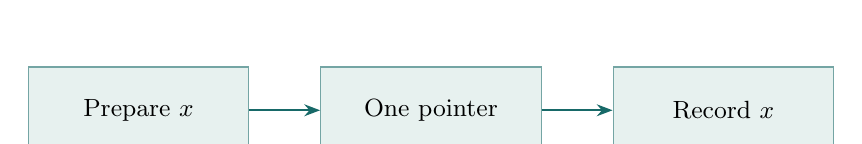
\begin{tikzpicture}[node distance=9mm]
\node[panel] (p) {\prepword\ $x$};\node[panel,right=of p] (m) {\pointerword};
\node[panel,right=of m] (r) {\recordword\ $x$};
\draw[link] (p)--(m);\draw[link] (m)--(r);
\end{tikzpicture}
\end{center}

In an operational model, a preparation is an instruction the laboratory can carry out. A test connects its output to allowed operations and ends with a record. Two preparations represent the same state precisely when every such test gives the same record, or the same distribution of records for probabilistic instruments. Adding a detector may separate preparations that were equivalent before.

\topic{A probability that counts a stopped branch}
Toss a fair coin. Select one branch and stop on the other. The probability recorded for selection is $1/2$. Normalizing over the surviving branch would answer a different question. A finite binary tree implements the experiment exactly. Sequential composition continues at each successful leaf. Parallel composition uses independent coins. Exchanging their order leaves closed probabilities unchanged.

The fixed pointer works with any finite number of symbols. A universal limit of seven needs an additional premise. An ontological question remains: what, besides their common responses, might operationally indistinguishable preparations share? UHM proposes a connection between physical organisation and experience. To turn such an interpretation into a prediction, one must say which further observation could distinguish it from another account.

\links{Finite laboratory, quotient by tests and exact probabilities: \href{https://github.com/gst-st/uhm/tree/main/website/research/operational-reconstruction/network}{OperationalProcess and RandomProcess}.}

\clearpage

\chaptertitle{Why seven occurs in one register}
Seven has a precise source in an error-correction problem. A word of $N$ binary symbols can arrive intact or with one flipped bit. Each such neighbourhood has $N+1$ words. If neighbourhoods around $M$ valid words are disjoint and exhaust all received words, then
\[
M(N+1)=2^N .
\]
For more than two valid words the first possible length is seven. Indeed $N+1$ must be a power of two. Lengths one and three have at most two words. At length seven the Hamming code attains the bound with sixteen valid words. This counts binary positions protecting a payload against one flip.

\topic{What the syndrome measures}
Assign each position a different nonzero column in $\mathbb F_2^3$. A single flip adds that column to the syndrome. Three distinct columns $a,b,c$ give zero syndrome exactly when $a+b+c=0$. The seven such triples form the lines of the Fano plane. A zero syndrome can therefore mean either no error or a three-bit pattern outside the promised noise class.

\begin{center}\begin{tabularx}{\linewidth}{@{}l>{\raggedright\arraybackslash}X>{\raggedright\arraybackslash}X@{}}\toprule
Experiment & Fixed input & Conclusion\\\midrule
One shared pointer & $n$ labelled outputs & $n$ distinct preparations\\
Perfect binary diagnosis & All zero- and one-flip records & Minimum length seven for $M>2$\\
Fano incidence & Two marked points & One line through the pair\\\bottomrule
\end{tabularx}\end{center}

An octonion table can use the same seven points. It additionally specifies signs for multiplication. Choosing an imaginary unit gives an $SU(3)$ stabilizer. Reading that stabilizer as colour requires a matter representation, transport between sites and field dynamics. Counting the three conjugate pairs of nonzero clock harmonics likewise leaves open whether a physical family occupies each pair.

\links{\href{https://holon.sh/docs/reference/premises}{Coding and matter premises}\quad
\href{https://holon.sh/docs/physics/gauge-symmetry/standard-model}{Gauge representations}\quad
\href{https://holon.sh/docs/physics/particle-physics/fermion-generations}{Clock harmonics}.}

\clearpage

\chaptertitle{Measuring distance by intervention}
Send a marked signal from $A$ to $B$, then relay it to $C$. Suppose the first segment costs two ticks and the second costs three. Relaying gives a five-tick protocol. To claim that the distance is five requires evidence that no faster allowed protocol succeeds. On a specified chain with a visible leading front and no alternative path, locality supplies the lower bound.\begin{center}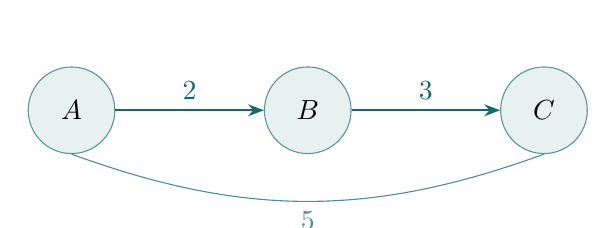
\begin{tikzpicture}
\foreach \x/\n in {0/A,3/B,6/C}{\node[draw=teal!70,fill=mist,circle,minimum size=11mm] (\n) at (\x,0) {$\n$};}
\draw[link] (A) -- node[above] {$2$} (B);\draw[link] (B) -- node[above] {$3$} (C);
\draw[teal!75] (A.south) to[bend right=20] node[below] {$5$} (C.south);
\end{tikzpicture}\end{center}

Let $d(a,b)$ be the least attainable transfer cost. The idle operation gives $d(a,a)=0$. If different sites have positive cost and concatenation costs no more than the sum, then $d(a,c)\le d(a,b)+d(b,c)$. Reversing a transfer at no greater cost gives symmetry. If acknowledgement takes two ticks in one direction and one in the other, the cost defines a directed distance. A physical device also needs a clock unit and a detection threshold.

\topic{Two probes can disagree}
Two probes may have different clock speeds. Their segment times must nevertheless have the same ratio if one positive scale factor per probe is to give a common geometry. For measured rows $(2,3)$ and $(2,4)$, the determinant is $2\cdot4-3\cdot2=2$. No change of either clock unit removes that disagreement. A common limiting geometry requires controlled comparisons as the network is refined. A three-site chain does not determine the dimension or gravitational dynamics of physical spacetime.

For a link $U_{ji}$ transporting matter from $i$ to $j$, a local frame change acts by $U_{ji}\mapsto g_j U_{ji}g_i^{-1}$. The middle frame cancels when two links compose. This covariance can be checked for a given group and transport rule. It leaves open which group acts in nature.

\links{\href{https://holon.sh/docs/geometry/response-metric}{Response metric}\quad
\href{https://holon.sh/docs/networks/three-node-transport}{Three-site transport}\quad
\href{https://holon.sh/docs/geometry/common-limit}{Common limiting geometry}.}

\clearpage

\chaptertitle{What a missing signal can hide}
Two paths reach the same receiver at the same time. Assume an experiment has established that their leading amplitudes add linearly. With one phase setting, the receiver sees $u+v$; with a calibrated sign reversal on the second arm it sees $u-v$. If both readings vanish then $2u=2v=0$. Thus two settings recover an arrival whenever at least one arm carries a nonzero amplitude, provided the detector can distinguish the resulting mode from its baseline.\begin{center}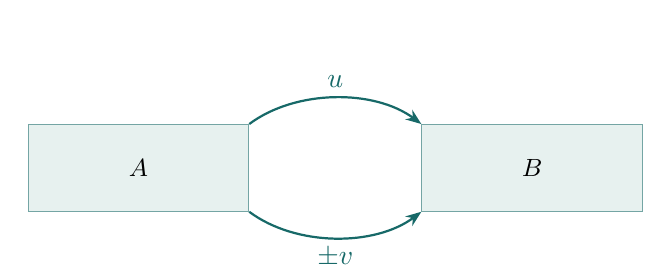
\begin{tikzpicture}
\node[panel] (a) at (0,0) {$A$};\node[panel] (b) at (5,0) {$B$};
\draw[link] (a.north east) .. controls (2,1.0) and (3,1.0) .. node[above] {$u$} (b.north west);
\draw[link] (a.south east) .. controls (2,-1.0) and (3,-1.0) .. node[below] {$\pm v$} (b.south west);
\end{tikzpicture}\end{center}

Here interference is a premise about preparations and joint detection. A table of possible routes alone does not imply linear addition, a complex phase or the Born rule. A real probability tree and a coherent two-arm setup can use the same connection diagram and have different readouts.

\topic{A phase-sensitive detector}
Within a complex seven-dimensional density model, prepare two matrices with diagonal entries $1/7$. Set every off-diagonal magnitude to $1/84$. Take all coherences real except $\rho_{12}=\pm i/84$ and its Hermitian conjugate. The matrices are strictly diagonally dominant: the sum of off-diagonal magnitudes in each row is $6/84<1/7$. Both are valid states. They are complex conjugates, so every real symmetric effect gives identical probabilities.

There is a direct way to reveal the difference. Use the projector onto $(|1\rangle+i|2\rangle)/\sqrt2$. Its two probabilities are $11/84$ and $13/84$. Comparing populations, magnitudes or spectra would miss the sign. This example states which operation supplies the missing information. It makes no claim that a given biological instrument measures that projector.

\links{\href{https://holon.sh/docs/networks/cycle-observations}{Closed paths and phase controls}\quad
\href{https://github.com/gst-st/uhm/blob/main/website/research/operational-reconstruction/verify_context.py}{Exact phase check}.}

\clearpage

\chaptertitle{Which geometry a matrix carries}
A finite complex quantum model assigns a Hermitian positive matrix of trace one to each preparation. A detector outcome is represented by an effect $E$, with probability $\operatorname{Tr}(E\rho)$. A deterministic process has a linear completely positive trace-preserving action; a general instrument has separate outcome branches. The assignment of these objects to an actual laboratory is part of the model.

The same matrix space allows different questions about closeness. For quantum fidelity $F(\rho,\sigma)=(\operatorname{Tr}\sqrt{\sqrt{\rho}\,\sigma\sqrt{\rho}})^2$, two conventions are the Bures angle $\arccos\sqrt F$ and the chordal distance $\sqrt{2-2\sqrt F}$. On two orthogonal pure states they give $\pi/2$ and $\sqrt2$. Both induce the usual finite-dimensional topology, but the numerical values and units of a distance threshold differ. A cost measured in ticks on a transmission network requires its own matching experiment.

\topic{Topology does not fix how preparations mix}
On density matrices the map $h(\rho)=\rho^2/\operatorname{Tr}(\rho^2)$ is continuous and invertible, with inverse $h^{-1}(\sigma)=\sqrt{\sigma}/\operatorname{Tr}\sqrt{\sigma}$. It preserves the topology. Yet a preparation made from three parts $|0\rangle$ to one part $|1\rangle$ has diagonal probabilities $(3/4,1/4)$, which the map changes to $(9/10,1/10)$. Applying the map to each pure state first and then mixing leaves $(3/4,1/4)$. The mixing experiment distinguishes the two descriptions.

A state encoder may also identify physically different histories. To use its output for prediction, one must check that histories with the same encoded state have the same future records under the allowed interventions. A symmetry of the target matrix space does not establish this property. To use a distance on rays as a distance between reported qualities, calibrate a map to reports and test new comparisons. The topology alone determines neither map.

\links{\href{https://holon.sh/docs/reference/mathematical-kernel}{Typed state space and observation closure}\quad
\href{https://holon.sh/docs/reference/notation}{Fidelity and distance conventions}.}

\clearpage

\chaptertitle{A model of experience needs a readout}
A person reports a sensation after a stimulus. The measured delay includes processes between the sensation and the report. Suppose the following synthetic data obey an additive law: each condition has an onset time $s_i$ and each reporting mode adds a delay $r_j$.

\begin{center}\begin{tabular}{@{}lrr@{}}\toprule
Time in ticks & Mode 1 & Mode 2\\\midrule
Condition 1 & 5 & 8\\
Condition 2 & 7 & 10\\\bottomrule\end{tabular}\end{center}

The rectangle contrast is $5+10-8-7=0$. The law fits with onset times $(4,6)$ and reporting delays $(1,4)$. It fits equally well with $(3,5)$ and $(2,5)$. All four observed times are identical in the two accounts. Turning the final 10 into 11 would instead make the contrast nonzero and reject exact additivity. With noisy data that decision needs repeat measurements and an uncertainty model. An independent reference is required to identify the absolute onset.

\topic{Where a numerical threshold belongs}
In a chosen seven-axis density model write $d=\sum_i\rho_{ii}^2$, $q=\sum_{i\ne j}|\rho_{ij}|^2$, $P=d+q$, $\Phi=q/d$ and $R=1/(7P)$. Normalization implies $d\ge1/7$. If the model selects $P>2/7$, $R\ge1/3$ and $\Phi\ge1$, then $q\ge d$ and $d+q\le3/7$. A normalized diagonal state supported equally on three axes has $P=1/3$ and $\Phi=0$. Passing one cut does not establish the others. An entropy score on a component also needs a declared component state.

These are conditions on matrices in a specified frame. To identify any of them with reported intensity, felt similarity or clinical well-being, fix the preparation and reporting protocol, calibrate the readout on one dataset, and predict a contrast under a new intervention. The ethical importance of a person's testimony does not depend on whether the proposed model fits it.

\links{\href{https://holon.sh/docs/reference/falsifiability}{Testing an experiential bridge}\quad
\href{https://holon.sh/docs/reference/specification}{State and readout definitions}.}

\clearpage

\chaptertitle{The cost of acting on a model}
A system that writes a new state after observing a record uses resources. Consider first an ordinary quantum device with a fixed environment, a fixed joint channel and an output obtained by discarding that environment. Its input--output map is affine: a random mixture of two preparations produces the corresponding mixture of the two outputs. A proposed nonlinear update calls for a different physical procedure.

\topic{An exact resource count}
Suppose a source can independently prepare repeated copies of
\[
 \rho_y=(1-y)I/7+y\Theta,\qquad 0\le y\le1,
\]
where the pure target $\Theta$ is known but $y$ is unknown. At fixed input rate parameter $\mu=1/2$, consider the model step $\rho_y\mapsto\rho_{g(y)}$ with
\[
 g(y)=\tfrac12+\tfrac12\,\frac{6y^3}{1+6y^2}.
\]
The device must announce success or failure. On success it must produce the specified state for every $y$. With three independent preparations a fixed instrument achieves this; two do not suffice. The optimal three-copy success probability on this family is $(1+6y^2)/7$. The probabilities at $y=0$ and $y=1$ are $1/7$ and $1$, respectively. Reporting only successes would hide this dependence.

The scope matters when discussing learning or agency. This is one feedback step on a commuting family, with a known target and repeatable preparations. It gives no implementation for an arbitrary unknown state, an unlimited supply of copies or an entire learning trajectory. A claim about memory needs distinct prior histories, their retained records, and a later task that distinguishes them.

\topic{What a monist interpretation asks}
Physical organisation and first-person description may concern the same underlying process. To investigate that possibility, keep distinct the response of an apparatus, a model of its internal state and a person's report. A bridge between them gains empirical content when it fixes a difference that an independent observation could reveal. Judgments about harm, consent and care require stated values as well as observations.

\links{\href{https://github.com/gst-st/uhm/blob/main/website/research/operational-reconstruction/feedback.md}{Feedback theorem and instrument}\quad
\href{https://holon.sh/docs/reference/status-registry}{Result registry}\quad
\href{https://holon.sh/docs/reference/mathematical-kernel}{Mathematical kernel}.}
\end{document}
